%%%%%%%%%%%%%%%%%%%%%%%%%%%%%%%%%%%%%%%%%%%%%%%%%%%%%%%%%%%%%%%%%%%%%%%%%%%%%%%%
% SD Lab -- Sockets
% Giovanni Ciatto
% Alma Mater Studiorum - Università di Bologna
% mailto:giovanni.ciatto@unibo.it
%%%%%%%%%%%%%%%%%%%%%%%%%%%%%%%%%%%%%%%%%%%%%%%%%%%%%%%%%%%%%%%%%%%%%%%%%%%%%%%%
%\documentclass[handout]{beamer}\mode<handout>{\usetheme{default}}
%
\documentclass[presentation]{beamer}\mode<presentation>{\usetheme{AMSBolognaFC}}
%\documentclass[handout]{beamer}\mode<handout>{\usetheme{AMSBolognaFC}}
%%%%%%%%%%%%%%%%%%%%%%%%%%%%%%%%%%%%%%%%%%%%%%%%%%%%%%%%%%%%%%%%%%%%%%%%%%%%%%%%
\usepackage{sd-lab-common}
\usepackage{sd-lab-sockets}
%%%%%%%%%%%%%%%%%%%%%%%%%%%%%%%%%%%%%%%%%%%%%%%%%%%%%%%%%%%%%%%%%%%%%%%%%%%%%%%%
\title[\currentLab{} -- Sockets]{Sockets}
%
\subtitle{\courseName{} (\courseAcronym) / Module \moduleN{}}
%
\author[\sspeaker{\gcShort} \& \mmShort]{
	\speaker{\gcFull} \and \mmFull
	\\ 
	\gcEmail \and \mmEmail
}
%
\institute[\disiShort, \uniboShort]{\disi{} (\disiShort)\\\unibo}
%
\date[A.Y. \academicYear{}]{Academic Year \academicYear{}}
%
%%%%%%%%%%%%%%%%%%%%%%%%%%%%%%%%%%%%%%%%%%%%%%%%%%%%%%%%%%%%%%%%%%%%%%%%%%%%%%%%
\begin{document}
%%%%%%%%%%%%%%%%%%%%%%%%%%%%%%%%%%%%%%%%%%%%%%%%%%%%%%%%%%%%%%%%%%%%%%%%%%%%%%%%

%\\\\\\\\\\\\\\\\\\\\\
\frame{\titlepage}
%\\\\\\\\\\\\\\\\\\\\\

\section{Overview}

\begin{frame}[c]{Motivation \& Lecture Goals}

Sockets are:
%
\begin{itemize}
	\item an ancient, and stable abstraction for low-level networking

	\vfill

	\item very general design/API, virtually supported by all major programming languages

	\vfill

	\item very didactic: they require a good understanding of DS fundamentals
    %
    \begin{itemize}
        \item[eg] client/server, or local/remote dichotomies
    \end{itemize}

	\vfill

	\item very elementary: higher-level communication abstractions can be built on top of them
	%
	\begin{itemize}
		\item[eg] RPC, HTTP, and virtually any application-level protocol
	\end{itemize}
\end{itemize}

\end{frame}

\begin{frame}[c]{Lab \labN{} Repository on GitLab}

	\begin{itemize}
		\item examples and exercises described in this lecture are provided by means of the following GitLab repository:
		%
		\begin{center}
			\url{\labRepo}
		\end{center}

		\vfill

		\item clone it on your machine using Git
		%
		\begin{itemize}
		    \item[\$] \texttt{git clone \textit{<repo URL>}}
		\end{itemize}

		\vfill

		\item even if a minimal environment simply relying on a text editor + Gradle is sufficient for this lab, we kindly suggest to import the cloned repository into some IDE, e.g. IntelliJ Idea or Eclipse

		\vfill

		\item in order to be able to submit your exercises, please ensure you requested access to the \href{\gitlabGroup}{GitLab group of the course}
	\end{itemize}

\end{frame}

\section{About Sockets}

\subsection{Overview}

\begin{frame}[c, allowframebreaks]{Overview}
    \begin{block}{Intuitive definition}
        A process's gateway towards the network, providing a full-duplex, multiplexable, point-to-point communication means towards other processes, distributed over the network
    \end{block}

    \begin{description}
        \item[distributed processes] --- sockets aims at letting \alert{processes} communicate, so
        %
        \begin{itemize}\small
            \item multiple processes on the same machine may communicate via sockets
            \item the same socket on the same machine may be shared among threads
        \end{itemize}

        \smallskip

        \item[communication] --- information exchange is \alert{explicit}
        %
        \begin{itemize}\small
            \item expect methods to send or receive data, explicitly
        \end{itemize}

        \smallskip

        \item[point-to-point] --- each socket mediates the interaction among \alert{two (and only two)} processes

        \smallskip

        \item[multiplexable] --- multiple independent sockets may be created, on different \alert{ports}
        %
        \begin{itemize}\small
            \item ports are positive 2-bytes integers in the range from 1 to $2^{16}-1$,
            \item the 1-1023 range is reserved for well-known protocols
            \item ports in the rage 1024-$2^{16}-1$ are for custom usage
        \end{itemize}

        \smallskip

        \item[full-duplex] --- exchanged data may flow in both verses simultaneously
        %
        \begin{itemize}\small
            \item[ie] the receiver may send data while receiving
            \item[ie] the sender may receive data while sending
        \end{itemize}

    \end{description}

    \framebreak

    \begin{block}{Two types of sockets}
        \begin{description}
            \item[stream sockets] allowing the exchange of \alert{possibly unlimited streams} of bytes
            %
            \begin{itemize}\small
                \item commonly based on TCP
                \item commonly operating in a \alert{connection-oriented} way
            \end{itemize}

            \item[datagram sockets] allowing the exchange of \alert{finite-sized packets} of bytes
            %
            \begin{itemize}\small
                \item commonly based on UDP
                \item commonly operating in a \alert{connectionless} way
            \end{itemize}
        \end{description}

        \smallskip

        \begin{itemize}
            \item in both cases, bytes are treated as \alert{opaque data}
        \end{itemize}
    \end{block}

    \framebreak

    Some jargon:

    \bigskip

    \begin{block}{Client vs. Server}
        \begin{description}
            \item[client socket] --- the one used to \alert{initiate} data exchange
            \item[server socket] --- the one used to \alert{wait} for data exchange to be initiated
        \end{description}
    \end{block}

    \bigskip

    \begin{block}{Local vs. remote}
        \begin{description}
            \item[local] $\approx$ on the \alert{current} side of a distributed interaction
            \item[remote] $\approx$ on the \alert{other} side of a distributed interaction
        \end{description}
    \end{block}
\end{frame}

\subsection{Stream sockets}

\begin{frame}[c, allowframebreaks]{Stream sockets}

    \begin{itemize}
        \item We focus on \alert{stream}, \alert{TCP}-based, \alert{connection-oriented} sockets\ldots
        %
        \begin{center}
            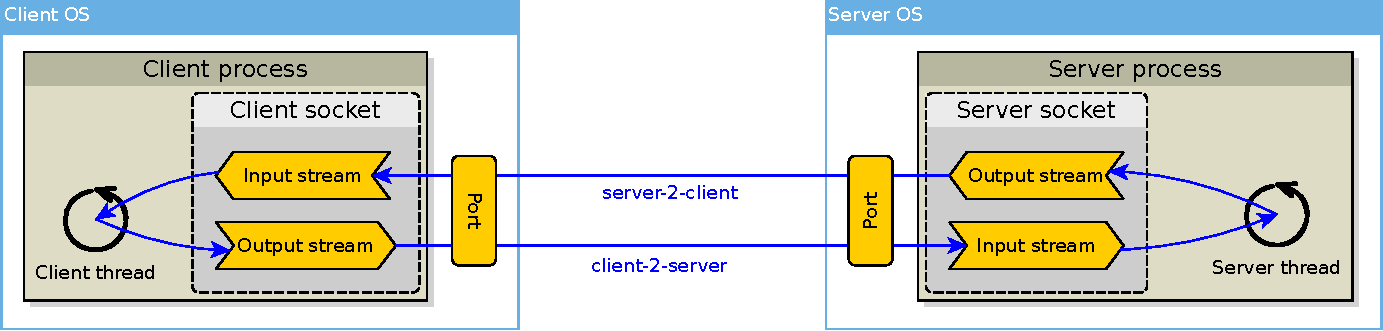
\includegraphics[width=\linewidth]{figures/sockets.pdf}
        \end{center}

        \smallskip

        \item \ldots which include two \alert{streams}:
        %
        \begin{description}\small
            \item[input stream] --- for receiving bytes from the remote host
            \item[output stream] --- for sending bytes to the remote host
        \end{description}

        \smallskip

        \item \ldots which require a TCP connection to be \alert{established} first
        %
        \begin{itemize}
            \item and eventually \alert{closed}, possibly gracefully
        \end{itemize}

        \smallskip

        \item \ldots which require a \alert{thread} to handle byte reception
    \end{itemize}

    \framebreak

    Three major phases in stream sockets usage:
    %
    \bigskip
    %
    \begin{enumerate}
        \item Establish a connection
        %
        \begin{enumerate}
            \item one server socket is used to \alert{listen} for incoming connections on a known \alert{port}
            \item one client socket is used to \alert{connect} to the first one
        \end{enumerate}

        \smallskip

        \item Exchange data
        %
        \begin{itemize}
            \item each end of the channel can \alert{receive} data by \alert{reading} on the \alert{input stream} \ldots
            \item \ldots or send data by \alert{writing} on the output stream of the local socket
            \item[!] the two operations can occur simultaneously
        \end{itemize}

        \smallskip

        \item Gracefully close the connection
        %
        \begin{itemize}
            \item either by closing the socket or both its streams
        \end{itemize}
    \end{enumerate}

\end{frame}

\subsubsection{Stream sockets in Java}

\begin{frame}[c, allowframebreaks]{Stream sockets in Java}

    Most relevant classes:
    %
    \bigskip
    %
    \begin{itemize}
        \item \texttt{java.net.\alert{Socket}} class for \alert{client} stream sockets \fnhint{\href{\javadoc{java/net/Socket.html}}{documentation of \texttt{Socket}}}
        %
        \begin{itemize}
            \item \alert{\texttt{new Socket()}} creates an unconntected socket
            \item \alert{\texttt{new Socket(\textit{String} host, \textit{int} port)}} creates a client socket and connects it to the remote end identified by \texttt{host:port}
            %
            \begin{itemize}
                \item host may be an host name (e.g. \texttt{www.google.it})
                \item or IPv4 address (e.g. \texttt{W.X.Y.Z})
            \end{itemize}
            \item \alert{\texttt{connect(\textit{SocketAddress} endpoint)}} attempts to connect this socket to \texttt{endpoint}
            %
            \begin{itemize}
                \item \texttt{endpoint} $\equiv$ remote hostname / address + port
                \item throws \texttt{IOException} in case of an error while connecting
            \end{itemize}

            \item \alert{\texttt{connect(\textit{SocketAddress} endpoint, \textit{int} timeout)}} like the above but throwing a \alert{SocketTimeoutException} if connection is not established within \texttt{timeout} milliseconds

            \item \alert{\texttt{getInputStream(): \textit{InputStream}}} returns the input stream of this socket

            \item \alert{\texttt{getOutputStream(): \textit{OutputStream}}} returns the output stream of this socket

            \item \alert{\texttt{close()}} closes the \texttt{Socket}, and the underlying TCP connection (therefore both the input and output streams)
            
            \item \alert{\texttt{shutdownInput()}} closes the \texttt{Socket}'s input stream alone
            
            \item \alert{\texttt{shutdownOutput()}} closes the \texttt{Socket}'s output stream alone
        \end{itemize}

        \framebreak

        \item \texttt{java.net.\alert{ServerSocket}} class for \alert{server} stream sockets \fnhint{\href{\javadoc{java/net/ServerSocket.html}}{documentation of \texttt{ServerSocket}}}
        %
        \begin{itemize}
            \item \alert{\texttt{new ServerSocket()}} creates an unbound server socket
            \item \alert{\texttt{new ServerSocket(\textit{int} port)}} creates a server socket and binds it to the local \texttt{port}
            %
            \begin{itemize}
                \item throws \texttt{IOException} if the port is already busy, or in case of error while binding
                \item throws \texttt{SecurityException} binding is prohibited for some reason
            \end{itemize}

            \item \alert{\texttt{bind(\textit{SocketAddress} endpoint)}} attempts to bind this socket to \texttt{endpoint}
            %
            \begin{itemize}
                \item \texttt{endpoint} $\equiv$ local hostname / address + port
                \item throws \texttt{IOException} in case of an error while connecting
            \end{itemize}

            \item \alert{\texttt{accept(): \textit{Socket}}} listens for a connection to be made to this socket and accepts it, returning a new \texttt{Socket} to be used to interact with the client
            %
            \begin{itemize}
                \item requires binding first
                \item this method is blocking! it returns only after a connection is established
            \end{itemize}

            \framebreak

            \item \alert{\texttt{getInputStream()}} as in \texttt{Socket}

            \item \alert{\texttt{getOutputStream()}} as in \texttt{Socket}

            \item \alert{\texttt{close()}} as in \texttt{Socket}
            
            \item \alert{\texttt{shutdownInput()}} as in \texttt{Socket}
            
            \item \alert{\texttt{shutdownOutput()}} as in \texttt{Socket}

        \end{itemize}

        \framebreak

        \item \texttt{java.net.\alert{InetSocketAddress}} a sub-type of \texttt{\textit{SocketAddress}}, represent a hostname/address + port couple \fnhint{\href{\javadoc{java/net/InetSocketAddress.html}}{documentation of \texttt{InetSocketAddress}}}
        %
        \begin{itemize}
            \item \alert{\texttt{new InetSocketAddress(\textit{int} port)}} any IP address on the local machine, on the specified \texttt{port}
            %
            \item \alert{\texttt{new InetSocketAddress(\textit{String} host, \textit{int} port)}} identifies the endpoint \texttt{host:port}
            %
            \begin{itemize}
                \item host may be an host name (e.g. \texttt{www.google.it})
                \item or IPv4 address (e.g. \texttt{W.X.Y.Z})
            \end{itemize}
        \end{itemize}

        \framebreak

        \item \texttt{java.io.\alert{InputStream}} base type for input streams \fnhint{\href{\javadoc{java/io/InputStream.html}}{documentation of \texttt{InputStream}}}
        %
        \begin{itemize}
            \item \alert{\texttt{read(\textit{byte[]} buffer): \textit{int}}} attempts to read \texttt{buffer.length} bytes from the stream, putting them in the \texttt{buffer}; returns the amount of bytes actually read
            %
            \begin{itemize}
                \item returns -1 if the the input stream is over
                \item blocks until some bytes can be read or the stream is closed
                \item throw \texttt{IOException} in case of problems (e.g. closed socket)
            \end{itemize}
            %
            \item \alert{\texttt{close()}} closes the input stream
            %
            \begin{itemize}
                \item throw \texttt{IOException} in case of problems
            \end{itemize}
        \end{itemize}

        \framebreak

        \item \texttt{java.io.\alert{OutputStream}} base type for output streams \fnhint{\href{\javadoc{java/io/OutputStream.html}}{documentation of \texttt{OutputStream}}}
        %
        \begin{itemize}
            \item \alert{\texttt{write(\textit{byte[]} buffer, \textit{int} offset, \textit{int} length)}} attempts to write \texttt{length} bytes into the stream, reading them from the \texttt{buffer}, starting from position \texttt{offset}
            %
            \begin{itemize}
                \item blocks until some bytes can actually be written
                \item throw \texttt{IOException} in case of problems (e.g. closed socket)
            \end{itemize}
            %
            \item \alert{\texttt{flush()}} forces previously written data to be actually written in the stream
            %
            \begin{itemize}
                \item (there may be some caching behind the scenes delaying writing of bytes)
            \end{itemize}
            %
            \item \alert{\texttt{close()}} closes the output stream
            %
            \begin{itemize}
                \item throw \texttt{IOException} in case of problems (e.g. closed socket)
            \end{itemize}
        \end{itemize}

    \end{itemize}

    \framebreak

    \begin{alertblock}{Counter-intuitive peculiarity of JDK}
        \begin{description}
            \item When an \texttt{Input}/\texttt{OutputStream} is actually owned by a \texttt{Socket}, its \texttt{\alert{close()}} actually closes the whole socket
            %
            \begin{itemize}
                \item so closing the input stream provokes the closure of the output stream
                \item and vice versa
            \end{itemize}
            \item You can use \texttt{OutputStream.}\alert{\texttt{shutdownInput}/\texttt{Output}()} instead
            %
            \begin{itemize}
                \item to selectively close one stream
            \end{itemize}
        \end{description}
    \end{alertblock}

\end{frame}

\begin{frame}[c, allowframebreaks]{Establishing a connection}

    In a nutshell:
    %
    \begin{center}
        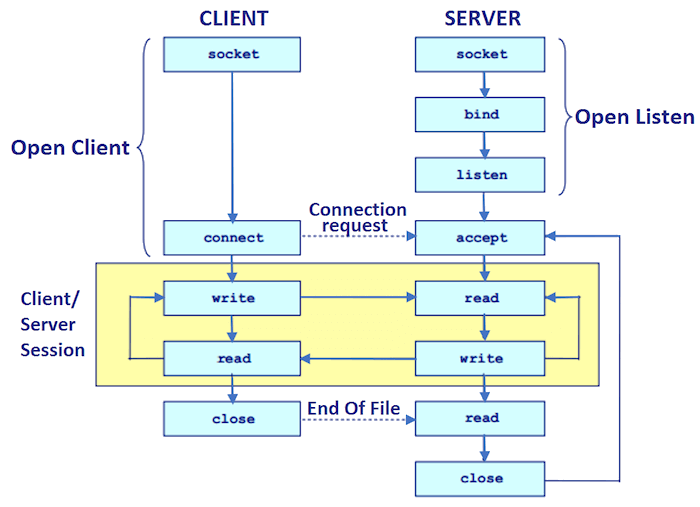
\includegraphics[width=.6\linewidth]{figures/socket-connection-overview.png}
    \end{center}

    \framebreak

    Detailed example: \hint{zoomable version \href{http://www.plantuml.com/plantuml/svg/nLLDRzim33rRlu9mWJK36cJ9iLY68aNH3IkQOktGIu52iPbQY2DbafoFVpzAjfmwKBSKE-oIs1RvI3xoKHV6ScshPSbE2v4Zp9MoCxLbPY7aYck-X8dQtl4y5_85XfyOeqD8lofZOPZ2oOruAUoah90bcP9MgnBkKQzHiuIyhSZ4YaiBq_iXiEGKPggIETSxk5VP0ks8iV4OZ7U0KXYBqeKPZnbBQXZeV_7Evm1fAd7JeDVklOzfoXAUMR7c5aDWoaGZlRV1EZui8JX2xNmaUEyZb6m3V-xt3sqqsafB-fkZHfaXM0KPBqjNROw7UGIaIB0qdGcPznwlRcwUlzzE7s-VxwO_7gBL91tNbWsDdZL2EW3n6AKzkLPbthJdMYFAc2K80tpDHSbd9OAI3fibVoN04DPQYTo5mj8WdDm9kNWhmAmoksEmRQ7Lna5FY9ghROOhrmuVG-RluTVHopFdtti7eytuqVnho9IKcBdm1fICSnoPicQaap1YuSkhuM9K2tbiNyjebB93iOpsQhei1KfB5YIKp3-7z5gba3qHsbZ2UH1AJ28jMZpvOGtMfZxi22DywzEv1pfU4stW5gIRS5DIBooMCuXheulMWlacZWXftpdG-Aj2Otr3qu2RDdI5haSTj5e6Zv7tYEifOFefrrHg4MHa2mI9TgFq0ZwuDus0Ms6i0GuhhJ8qVh24tI-zjmQD9VKqnKf4OocaC0Nci16sw6PT5xhlvJ6-WQD8hsFo9qEfB89sj82QDwRdmKMO49AYIBKvUv9SvewiVES6HKYBchfAE9rLSiabuJfVIwTGA6DzaaA25KjKbNsZlexVCIMrMwS-VQZHE-idOKrkeVjyTspp9pyVN9CBRa0gVy-93F-jvoIqoc0UgJzg5wRvU2A-JLzNxxTlLCdj9gF59EgobyZbfX0j3-5cDo97MbN_NKdTjKn5krlOpI6k2boYvYMibBPFik6HZWAvxUPgAFU5_N7zEJaC1k4Y6WpYLvYNJubphvw06XwEbWzpJRgWdsfP_WO0}{here}}
    %
    \begin{center}
        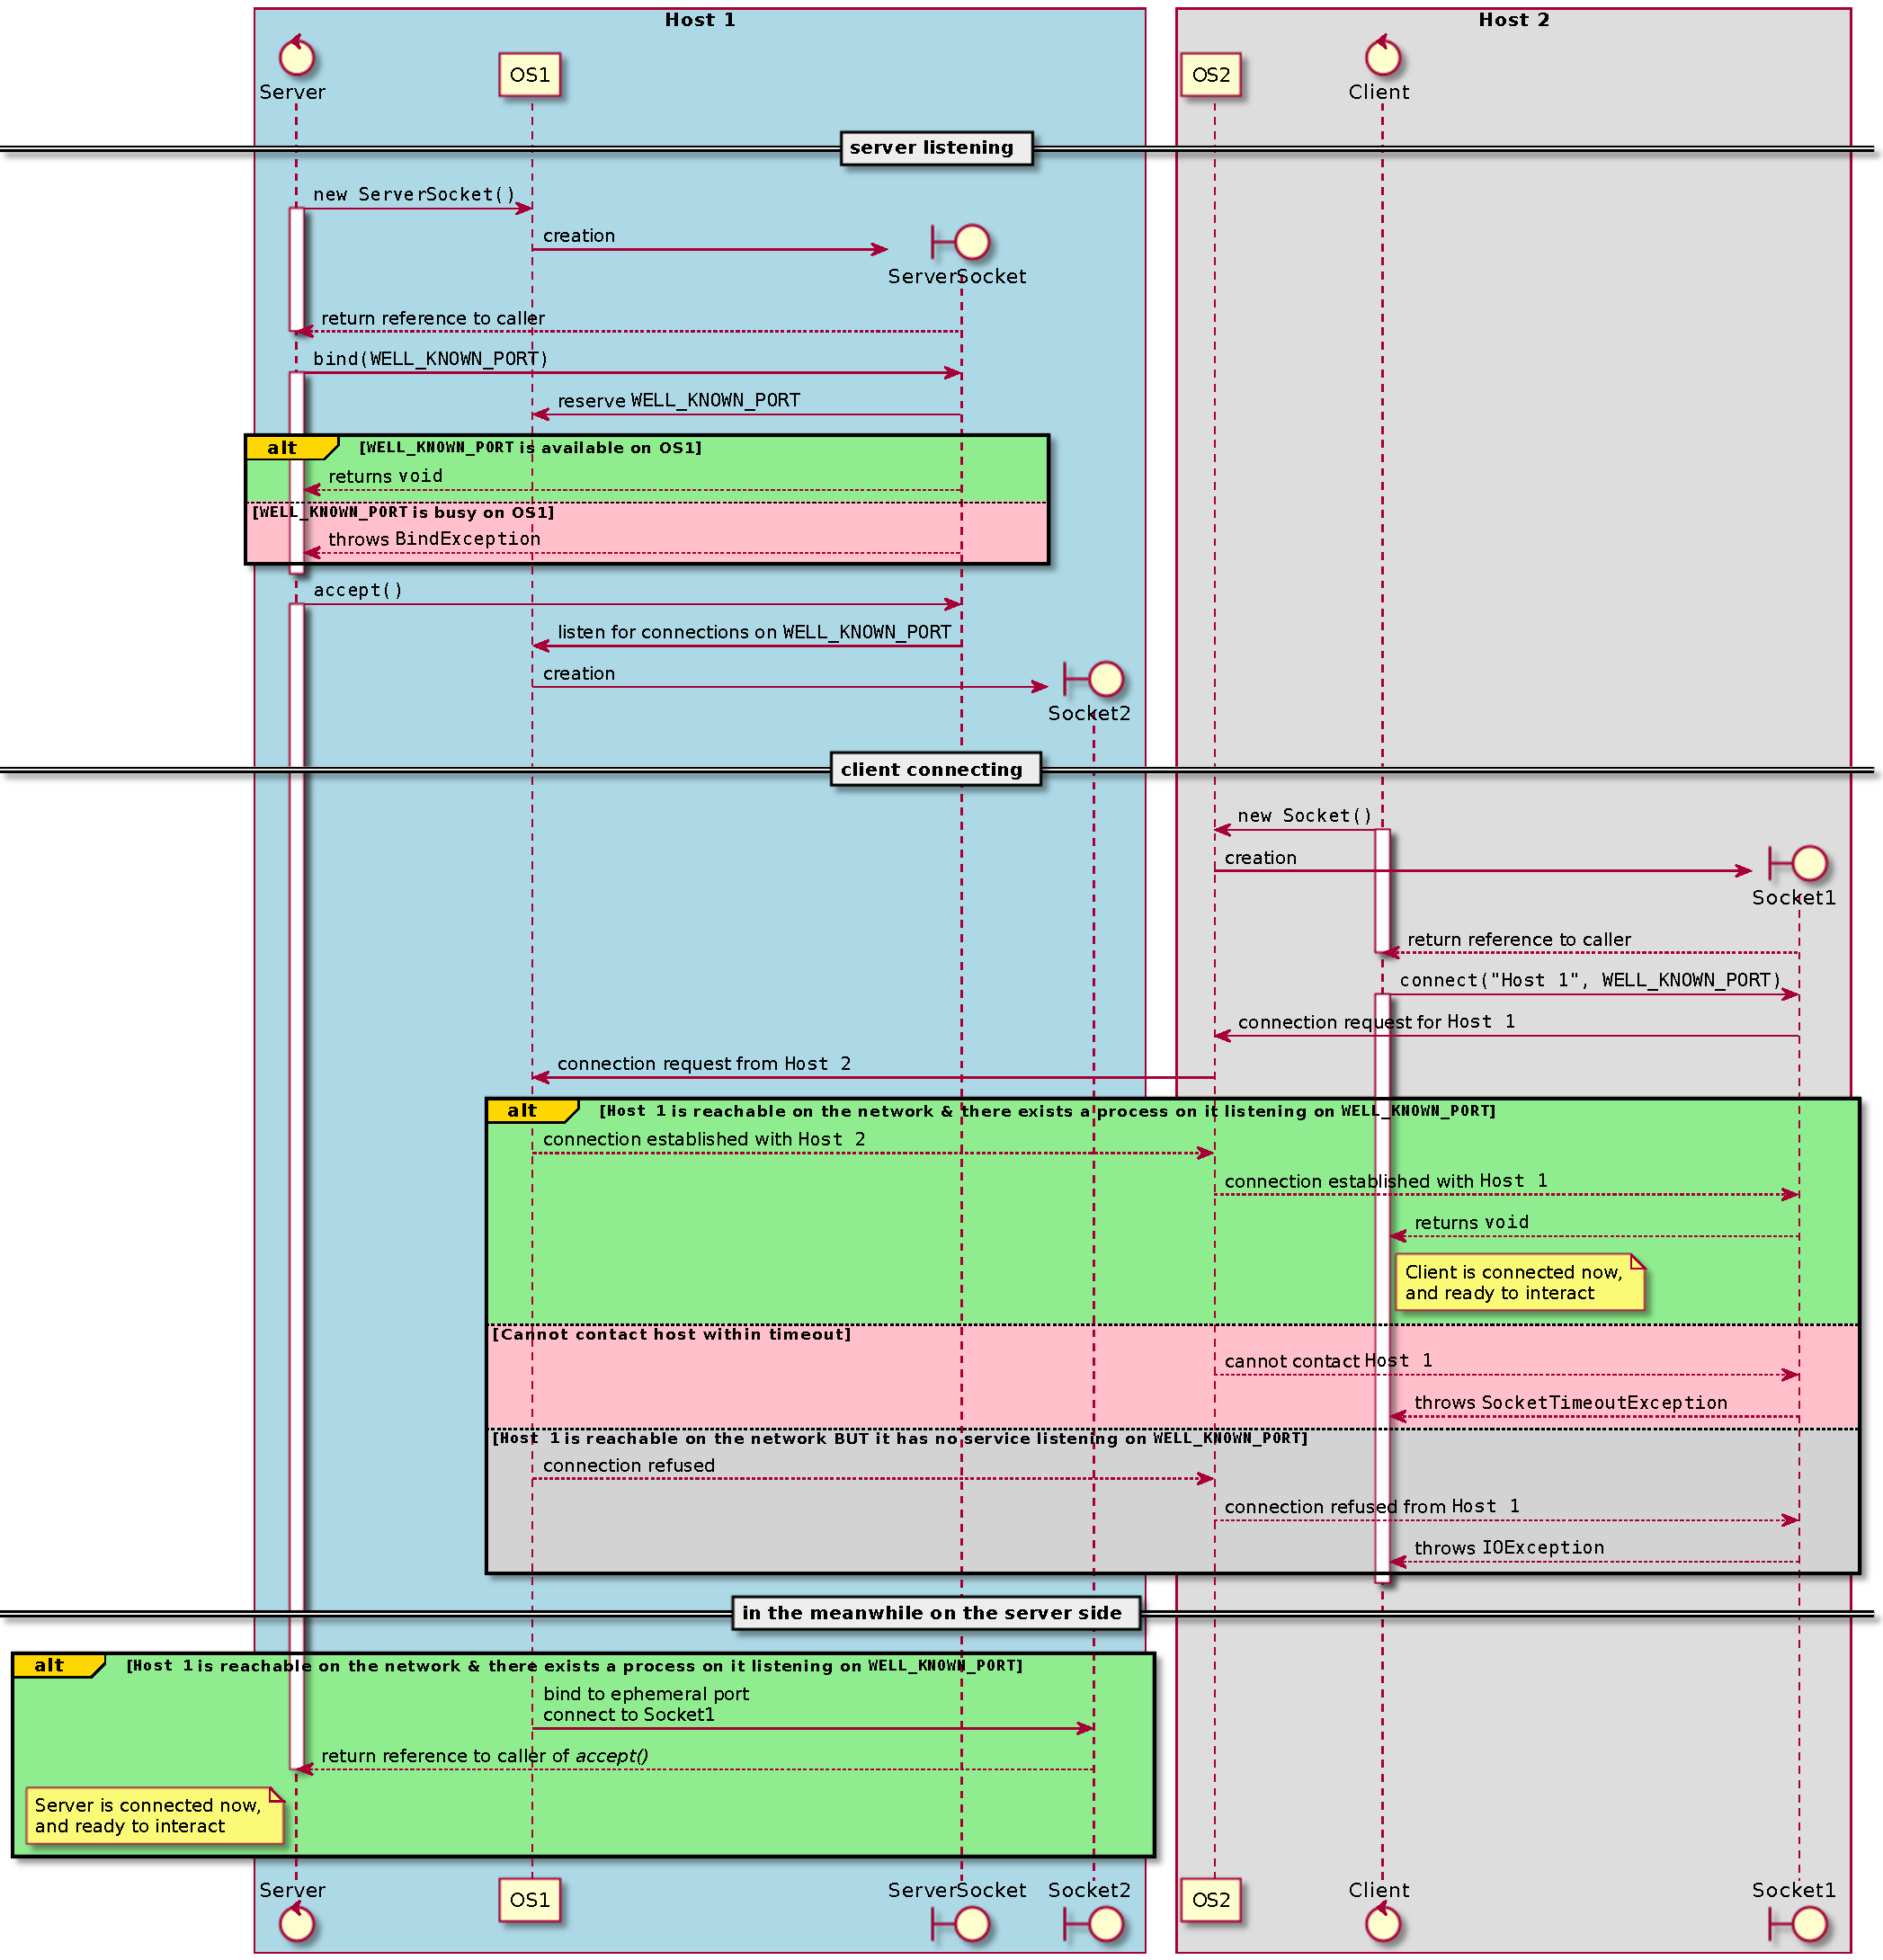
\includegraphics[width=.5\linewidth]{figures/sockets-connection.pdf}
    \end{center}

\end{frame}

\begin{frame}[c, allowframebreaks]{Reading and writing data with sockets}

    Reading a \alert{stream of bytes} from a socket:
    %
    \lstinputlisting[language=Java]{listings/bufferedRead.java}
    %
    \begin{itemize}
        \item here we suppose some callbacks are handling the read bytes
        %
        \begin{itemize}
            \item callbacks invocations are placeholders for actual business logic
        \end{itemize}

        \item developers may choose to either:
        %
        \begin{itemize}
            \item process the read bytes progressively
            \item or read it all, store it in memory, and process it as a whole
        \end{itemize}
    \end{itemize}

    \framebreak

    Writing a \alert{byte array} into a socket:
    %
    \lstinputlisting[language=Java]{listings/writeData.java}
    %
    %
    \begin{itemize}
        \item developers should find a way to encode their data structures into byte arrays
    \end{itemize}

\end{frame}

\section{Check Your Understanding}

\subsection{Sequential Echo Server}

\begin{frame}[c,allowframebreaks]{Example -- Sequential Echo Service}

    \begin{block}{Requirements -- Server side}
        \begin{itemize}
            \item A server process listening on port $P$ for TCP connection
            \item It accepts TCP requests and handles them \alert{sequentially}
            %
            \begin{itemize}
                \item hence, once it accepts one connection it ignores any other connection attempt\ldots
                \item \ldots until the current connection is closed by the client
            \end{itemize}
            \item While the current connection is open, it simply echoes the input stream
            %
            \begin{itemize}
                \item[ie] the input stream data is copied onto the output stream
            \end{itemize}
            \item Echoing goes on until the client closes the connection
            %
            \begin{itemize}
                \item or simply until its stream is over
            \end{itemize}
            \item If the local input stream is closed, then
            %
            \begin{itemize}
                \item any currently open connection is forcedly closed
                \item the server process is terminated
            \end{itemize}
        \end{itemize}
    \end{block}

    \begin{block}{Requirements -- Client side}
        \begin{itemize}
            \item A client process willing to connect to host $H$ on port $P$
            \item It initiates TCP connections towards $H$:$P$
            \item It sends any data read from the local standard input toward the socket
            \item It prints any data read from the socket to the local standard output
            \item It closes the connection whenever the standard input is closed
            %
            \begin{itemize}
                \item in that case, the client process is terminated as well
            \end{itemize}
        \end{itemize}
    \end{block}

    \begin{alertblock}{About input streams and threads}
        \begin{itemize}
            \item Beware that several input streams are involved, for each process
            \item This implies that each process should involve multiple threads
            \item This is due the input stream reading being blocking
        \end{itemize}
    \end{alertblock}

    \begin{center}
        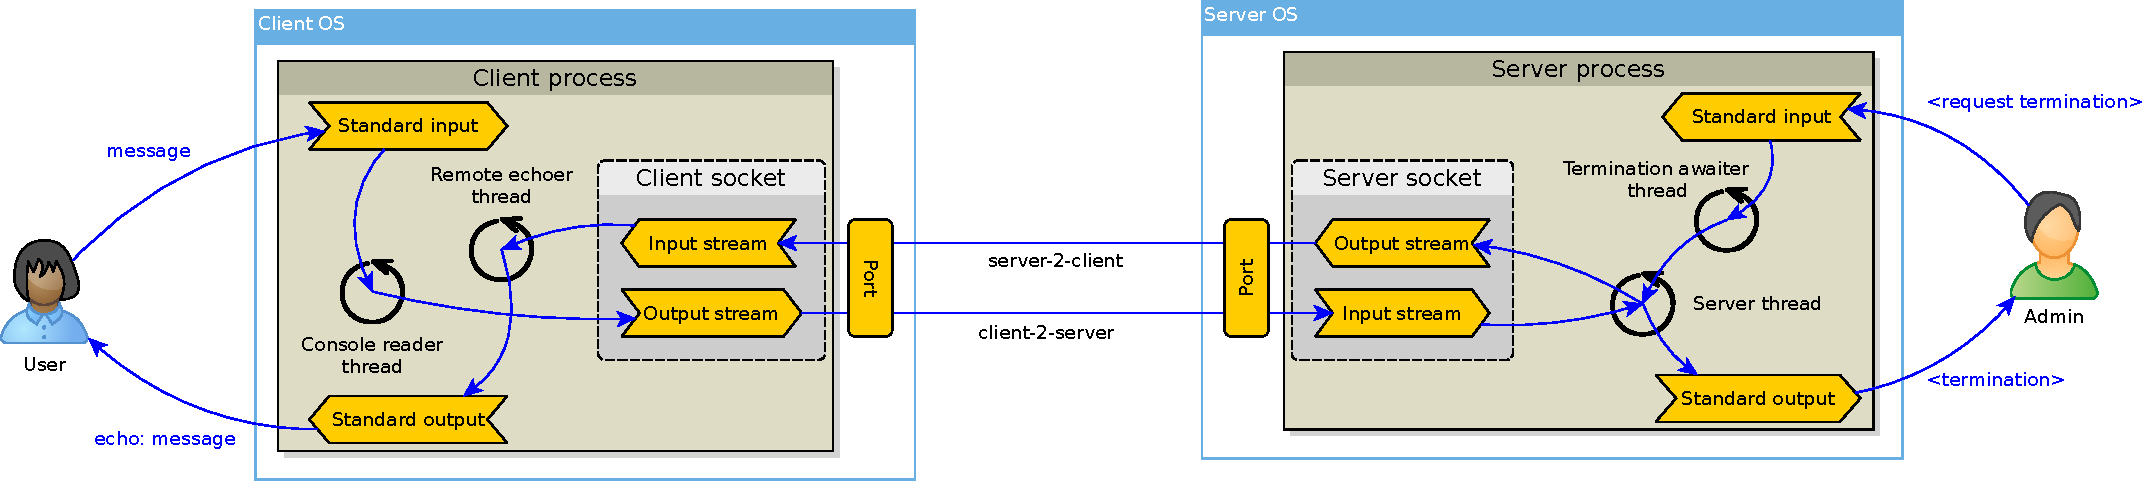
\includegraphics[width=\linewidth]{figures/echoer.pdf}
    \end{center}

\end{frame}

\subsection{Concurrent Echo Server}

\startExercise

\begin{frame}[c,allowframebreaks]{Exercise \currentExercise{} -- Concurrent Echo Server}

    \begin{alertblock}{Mandatory exercise}
        \begin{itemize}
            \item This exercise is mandatory
            \item Its submission and understanding will be certainly checked before the final exam
        \end{itemize}
    \end{alertblock}

    \begin{block}{Activity}
        Extend the sequential echo service example in such a way that
        %
        \begin{enumerate}
            \item Multiple connections can be simultaneously handled by the service
            %
            \item Shut-down of both client and server is gracefully handled
            %
            \begin{itemize}
                \item expected disconnections do not print exceptions
                \item unexpected disconnections do print exceptions
                \item binding/connection issues do print exceptions and stop the process
            \end{itemize}

            \item All automated tests are satisfied
        \end{enumerate}
    \end{block}

\end{frame}


%===============================================================================
\section*{}
%===============================================================================

%\\\\\\\\\\\\\\\\\\\\\
\frame{\titlepage}
%\\\\\\\\\\\\\\\\\\\\\

%%===============================================================================
%\section*{\refname}
%%===============================================================================
%
%%\\\\\\\\\\\\\\\\\\\\\
%%%%%
%%\begin{frame}[t,allowframebreaks]\scriptsize
%\begin{frame}[c]\footnotesize
%\frametitle{\refname}
%\bibliographystyle{apalike}
%\bibliography{sd-lab-sockets}
%\end{frame}
%%\\\\\\\\\\\\\\\\\\\\\

%%%%%%%%%%%%%%%%%%%%%%%%%%%%%%%%%%%%%%%%%%%%%%%%%%%%%%%%%%%%%%%%%%%%%%%%%%%%%%%
\end{document}
%%%%%%%%%%%%%%%%%%%%%%%%%%%%%%%%%%%%%%%%%%%%%%%%%%%%%%%%%%%%%%%%%%%%%%%%%%%%%%%%

